\documentclass[12pt, a4paper]{article}


% A pretty common set of packages
\usepackage[margin=2.5cm]{geometry}
\usepackage[T1]{fontenc}
\usepackage{graphicx}
\usepackage{amssymb}
\usepackage{amsmath}
\usepackage{bm}
\usepackage{color}
\usepackage{float}
\usepackage{bm}
\usepackage{physics}
\usepackage{subcaption}

\DeclareRobustCommand{\uvec}[1]{{%
  \ifcsname uvec#1\endcsname
     \csname uvec#1\endcsname
   \else
    \bm{\hat{\mathbf{#1}}}%
   \fi
}}
\newcommand{\olsi}[1]{\,\overline{\!{#1}}} % overline short italic

\usepackage[colorlinks=true, 
    linkcolor=blue,          % color of internal links
    citecolor=blue,        % color of links to bibliography
    filecolor=blue,      % color of file links
    urlcolor=blue]{hyperref}

\title{[16-833] Homework 3 : Written Report}
\author{Bharath Somayajula}
\date{\today}

\begin{document}

\maketitle

\tableofcontents
\section{Linear SLAM}
\subsection{Odometry}
\subsubsection{Measurement Function}
Since the odometry results in a change in position, the measurement function is simply
\[h_o(\mathbf{r}^t, \mathbf{r}^{t+1}) = \mathbf{r}^{t+1} - \mathbf{r}^t\]
\subsubsection{Jacobian}
The Jacobian of measurement function is
\[H_o(\mathbf{r}^t, \mathbf{r}^{t+1}) = \begin{bmatrix}
  -1 & 0 & 1 & 0\\
  0 & -1 & 0 & 1\\
\end{bmatrix}\]
\subsection{Landmark}
Since landmarks are measured using the relative position of the robot and landmark, the measurement function is simply
\[h_l(\mathbf{r}^t, \mathbf{l}^{k}) = \mathbf{l}^{k} - \mathbf{r}^t\]
\subsubsection{Jacobian}
The Jacobian of measurement function is
\[H_l(\mathbf{r}^t, \mathbf{l}^{k}) = \begin{bmatrix}
  -1 & 0 & 1 & 0\\
  0 & -1 & 0 & 1\\
\end{bmatrix}\]
\subsection{Results for \textit{2d\_linear.npz}}
\subsubsection{\textit{default}}

\begin{figure}[H]
  \centering
  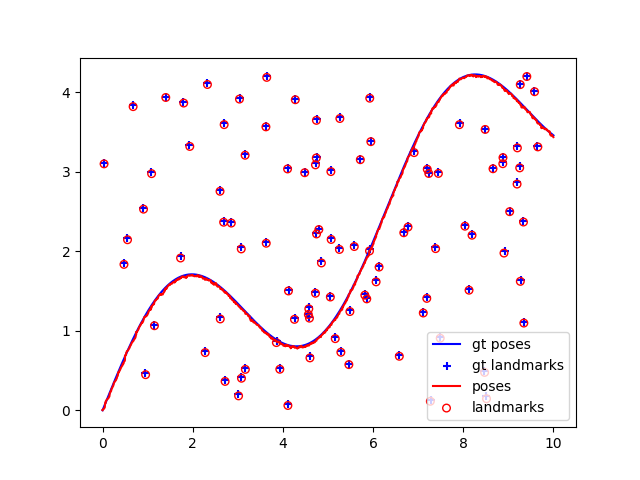
\includegraphics[width=0.8\textwidth]{./results/linear/default_2d_linear_map.png}
  \caption{Results with \textit{default}}
\end{figure}
\subsubsection{\textit{pinv}}

\begin{figure}[H]
  \centering
  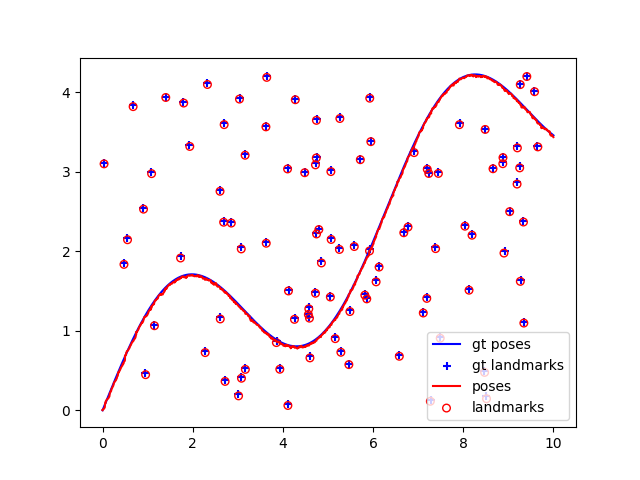
\includegraphics[width=0.8\textwidth]{./results/linear/pinv_2d_linear_map.png}
  \caption{Results with \textit{pinv}}
\end{figure}
\subsubsection{\textit{lu}}
\begin{figure}[H]
  \centering
  \begin{subfigure}[b]{0.45\textwidth}
    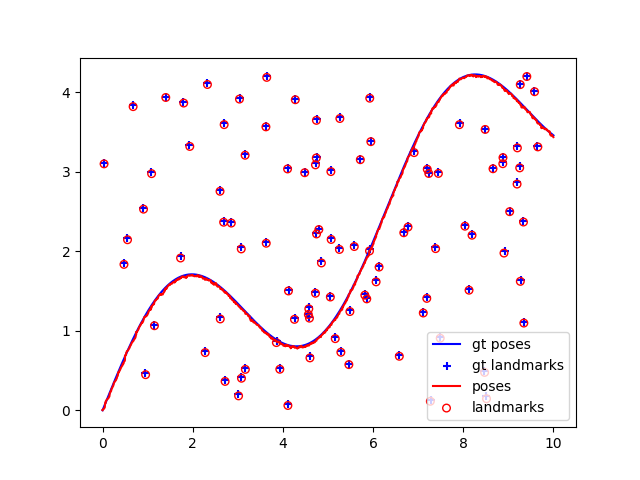
\includegraphics[width=\textwidth]{./results/linear/lu_2d_linear_map.png}
    \caption{Map}
  \end{subfigure}
  \hfill
  \begin{subfigure}[b]{0.45\textwidth}
    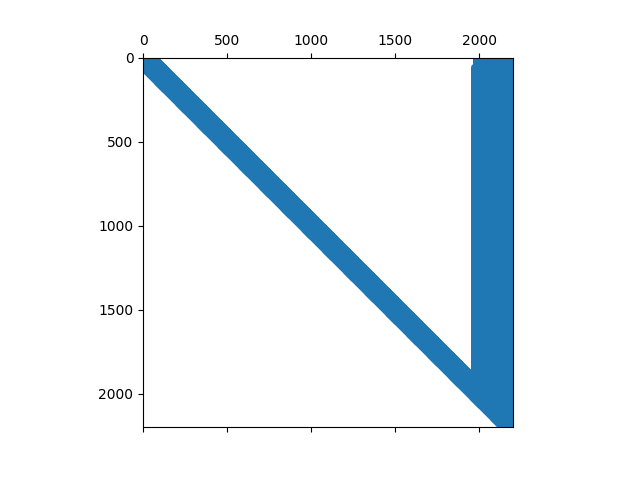
\includegraphics[width=\textwidth]{./results/linear/lu_2d_linear_sparsity.png}
    \caption{Sparsity}
  \end{subfigure}
  \caption{Results with \textit{lu}}
\end{figure}
\subsubsection{\textit{qr}}
\begin{figure}[H]
  \centering
  \begin{subfigure}[b]{0.45\textwidth}
    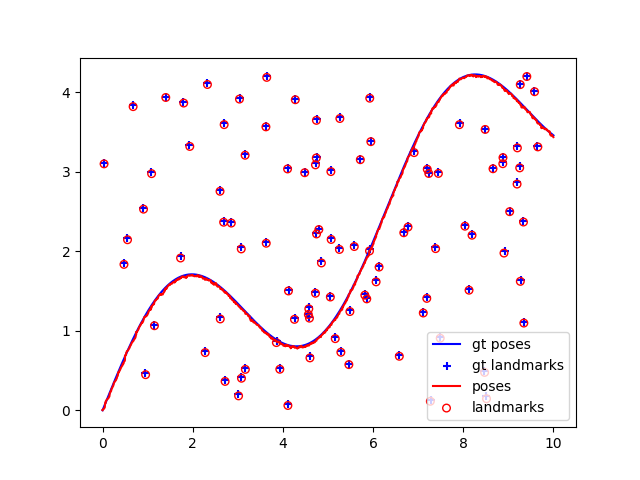
\includegraphics[width=\textwidth]{./results/linear/qr_2d_linear_map.png}
    \caption{Map}
  \end{subfigure}
  \hfill
  \begin{subfigure}[b]{0.45\textwidth}
    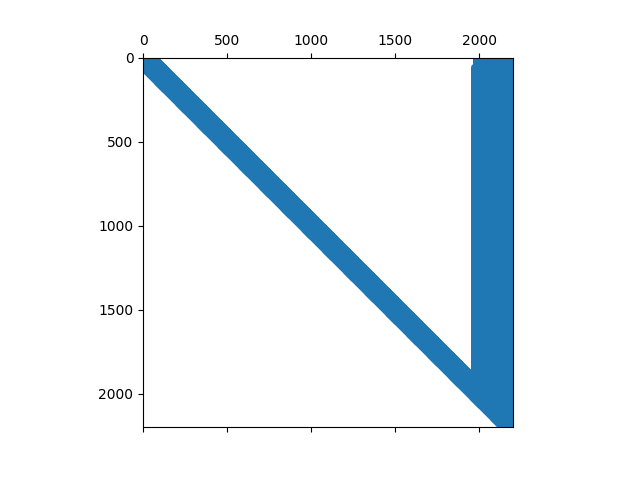
\includegraphics[width=\textwidth]{./results/linear/qr_2d_linear_sparsity.png}
    \caption{Sparsity}
  \end{subfigure}
  \caption{Results with \textit{qr}}
\end{figure}
\subsubsection{\textit{lu\_colamd}}
\begin{figure}[H]
  \centering
  \begin{subfigure}[b]{0.45\textwidth}
    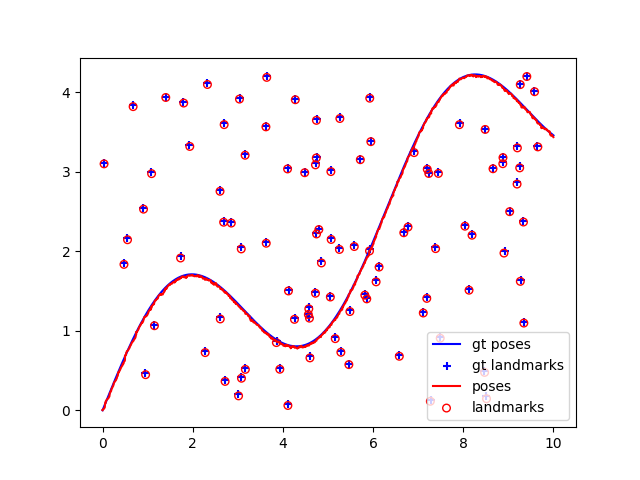
\includegraphics[width=\textwidth]{./results/linear/lu_colamd_2d_linear_map.png}
    \caption{Map}
  \end{subfigure}
  \hfill
  \begin{subfigure}[b]{0.45\textwidth}
    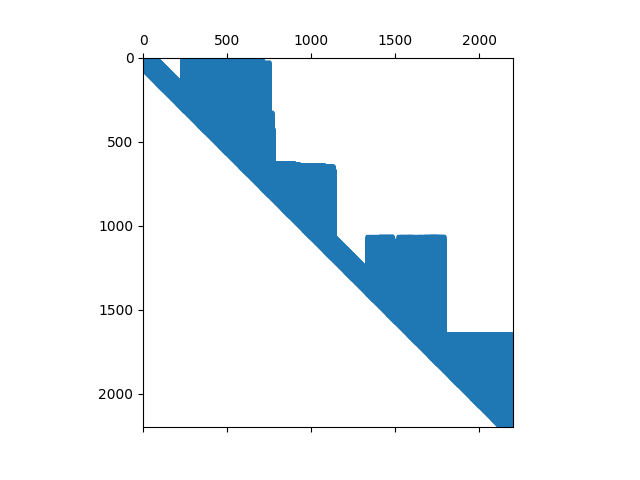
\includegraphics[width=\textwidth]{./results/linear/lu_colamd_2d_linear_sparsity.png}
    \caption{Sparsity}
  \end{subfigure}
  \caption{Results with \textit{lu\_colamd}}
\end{figure}
\subsubsection{\textit{qr\_colamd}}
\begin{figure}[H]
\centering
\begin{subfigure}[b]{0.45\textwidth}
  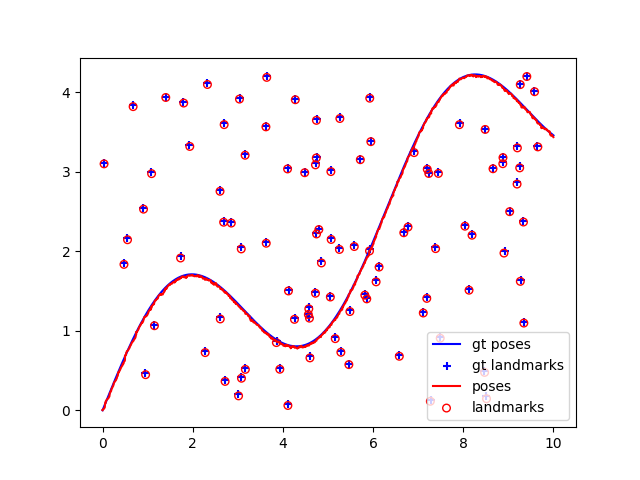
\includegraphics[width=\textwidth]{./results/linear/qr_colamd_2d_linear_map.png}
  \caption{Map}
\end{subfigure}
\hfill
\begin{subfigure}[b]{0.45\textwidth}
  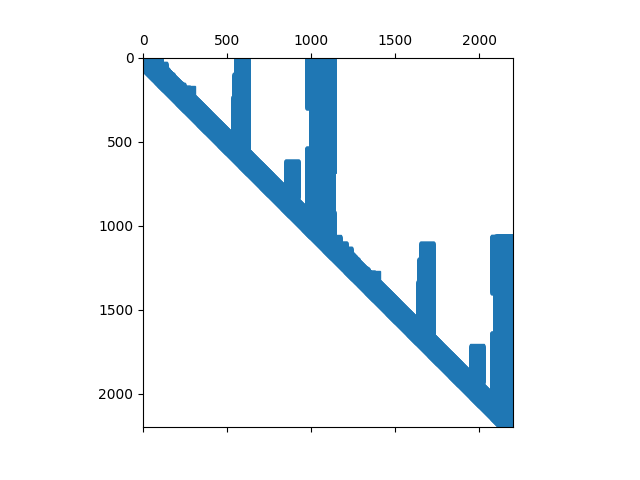
\includegraphics[width=\textwidth]{./results/linear/qr_colamd_2d_linear_sparsity.png}
  \caption{Sparsity}
\end{subfigure}
\caption{Results with \textit{qr\_colamd}}
\end{figure}
\subsubsection{Time}
\begin{table}[H]
  \centering
  \begin{tabular}{|c|c|c|}
  \hline
  \textbf{Method} & \textbf{Time(ms)}\\
  \hline
  \textit{default} & 32\\\hline
  \textit{pinv} & 1268\\\hline
  \textit{lu} & 288\\\hline
  \textit{qr} & 15\\\hline
  \textit{lu\_colamd} & 255\\\hline
  \textit{qr\_colamd} & 35\\\hline
  \hline
  \end{tabular}
  \caption{Optimization time for each method in milliseconds}
  \end{table}
\subsubsection{Conclusions}
\begin{enumerate}
  \item The \textit{pinv} method is the slowest since it involves computation of matrix inverse
  \item The \textit{qr} method is faster than \textit{lu} since QR factorization takes advantage of sparsity of input matrix during factorization process

\end{enumerate}
\subsection{Results for \textit{2d\_linear\_loop.npz}}
\subsubsection{\textit{default}}
\begin{figure}[H]
  \centering
  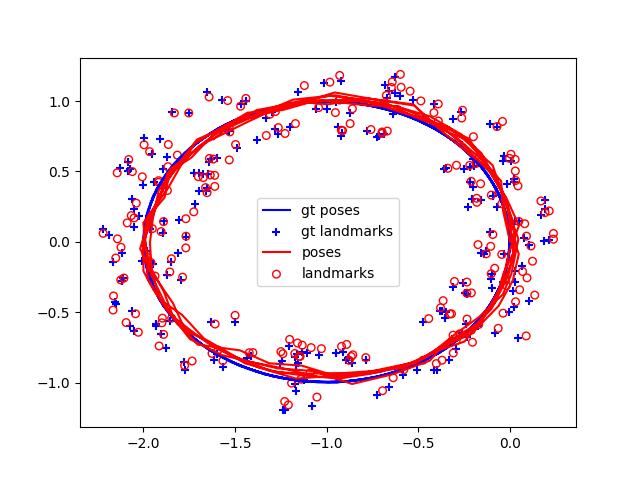
\includegraphics[width=0.8\textwidth]{./results/linear/default_2d_linear_loop_map.png}
  \caption{Results with \textit{default}}
\end{figure}
\subsubsection{\textit{pinv}}
\begin{figure}[H]
  \centering
  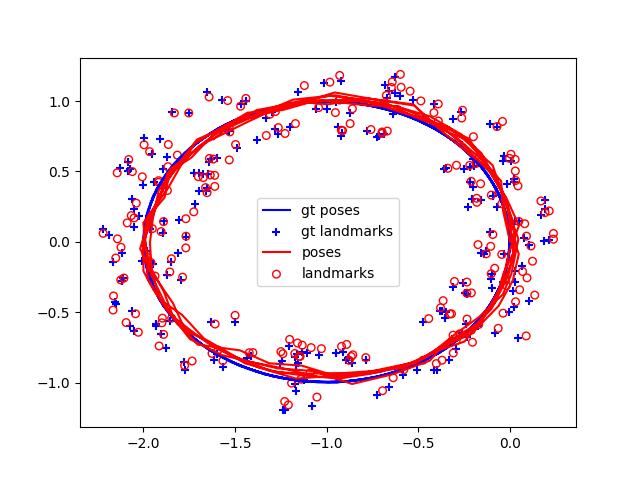
\includegraphics[width=0.8\textwidth]{./results/linear/pinv_2d_linear_loop_map.png}
  \caption{Results with \textit{pinv}}
\end{figure}
\subsubsection{\textit{lu}}
\begin{figure}[H]
  \centering
  \begin{subfigure}[b]{0.45\textwidth}
    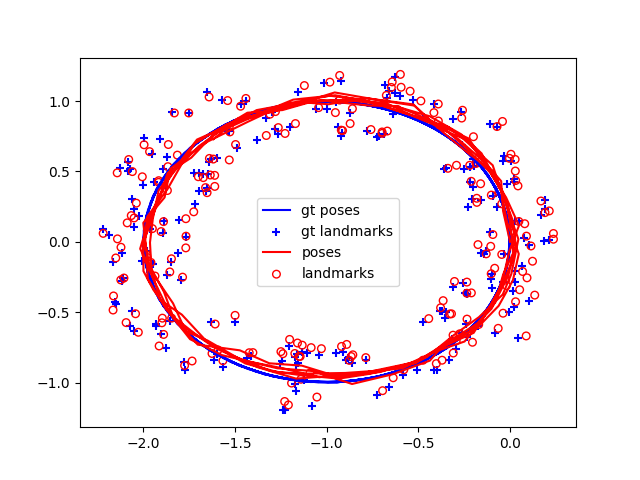
\includegraphics[width=\textwidth]{./results/linear/lu_2d_linear_loop_map.png}
    \caption{Map}
  \end{subfigure}
  \hfill
  \begin{subfigure}[b]{0.45\textwidth}
    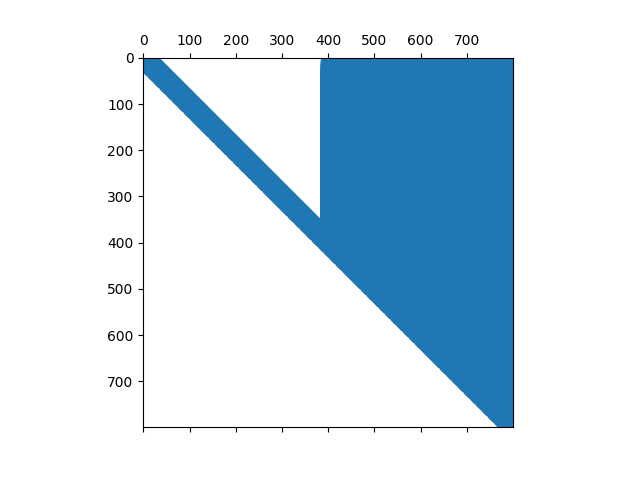
\includegraphics[width=\textwidth]{./results/linear/lu_2d_linear_loop_sparsity.png}
    \caption{Sparsity}
  \end{subfigure}
  \caption{Results with \textit{lu}}
\end{figure}
\subsubsection{\textit{qr}}
\begin{figure}[H]
  \centering
  \begin{subfigure}[b]{0.45\textwidth}
    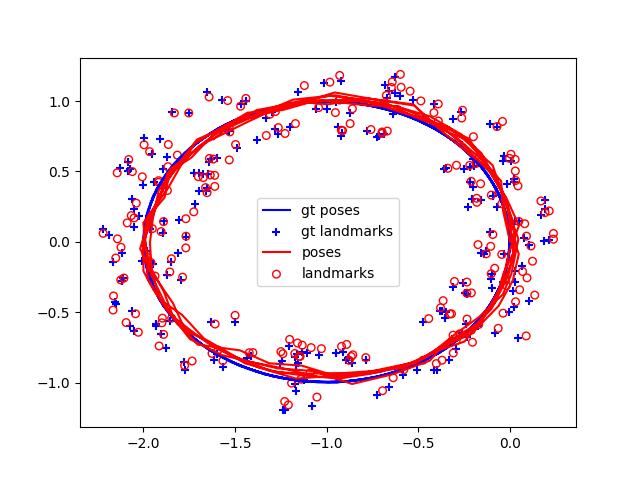
\includegraphics[width=\textwidth]{./results/linear/qr_2d_linear_loop_map.png}
    \caption{Map}
  \end{subfigure}
  \hfill
  \begin{subfigure}[b]{0.45\textwidth}
    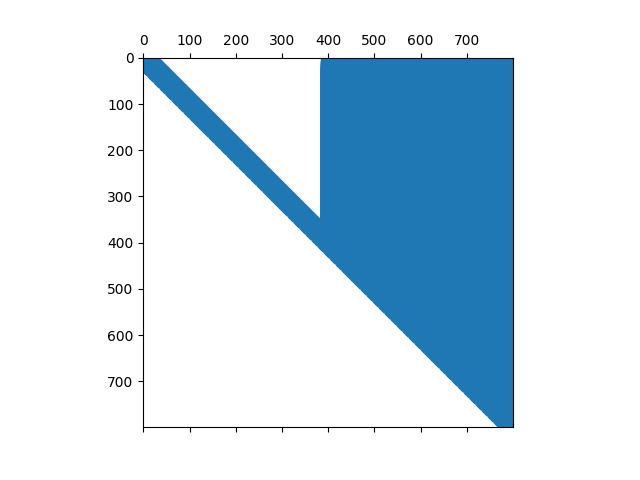
\includegraphics[width=\textwidth]{./results/linear/qr_2d_linear_loop_sparsity.png}
    \caption{Sparsity}
  \end{subfigure}
  \caption{Results with \textit{qr}}
\end{figure}
\subsubsection{\textit{lu\_colamd}}
\begin{figure}[H]
  \centering
  \begin{subfigure}[b]{0.45\textwidth}
    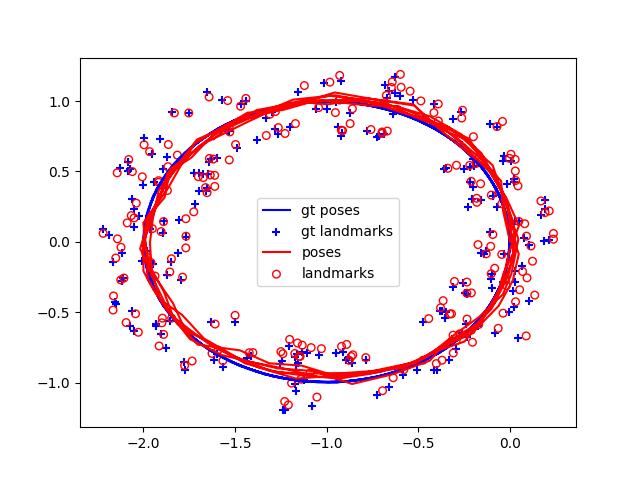
\includegraphics[width=\textwidth]{./results/linear/lu_colamd_2d_linear_loop_map.png}
    \caption{Map}
  \end{subfigure}
  \hfill
  \begin{subfigure}[b]{0.45\textwidth}
    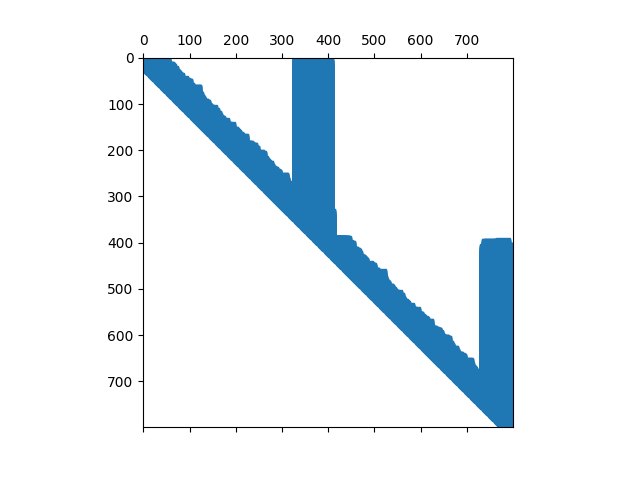
\includegraphics[width=\textwidth]{./results/linear/lu_colamd_2d_linear_loop_sparsity.png}
    \caption{Sparsity}
  \end{subfigure}
  \caption{Results with \textit{lu\_colamd}}
\end{figure}
\subsubsection{\textit{qr\_colamd}}
\begin{figure}[H]
\centering
\begin{subfigure}[b]{0.45\textwidth}
  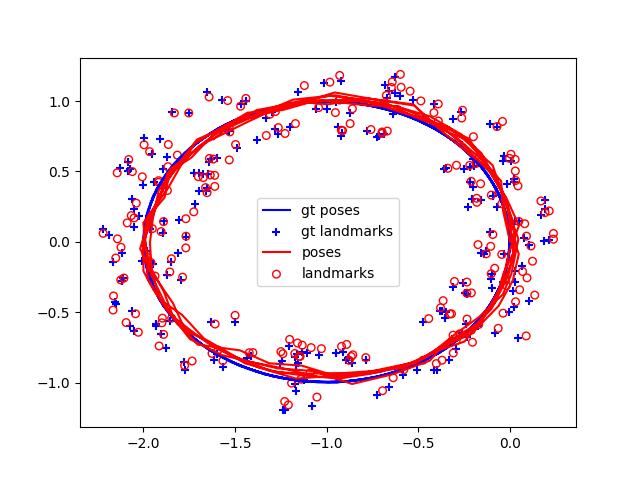
\includegraphics[width=\textwidth]{./results/linear/qr_colamd_2d_linear_loop_map.png}
  \caption{Map}
\end{subfigure}
\hfill
\begin{subfigure}[b]{0.45\textwidth}
  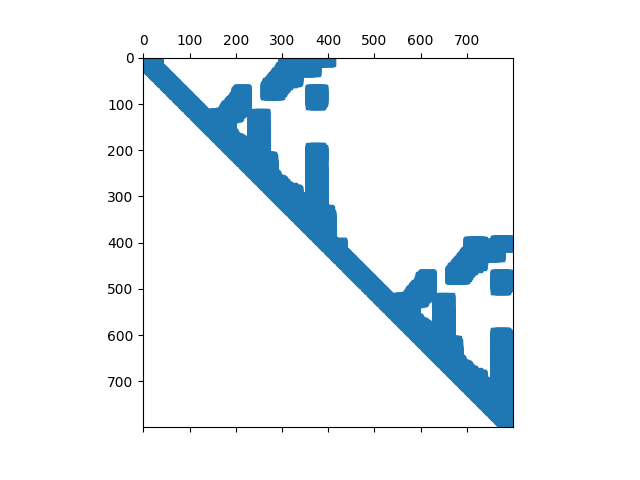
\includegraphics[width=\textwidth]{./results/linear/qr_colamd_2d_linear_loop_sparsity.png}
  \caption{Sparsity}
\end{subfigure}
\caption{Results with \textit{qr\_colamd}}
\end{figure}
\subsubsection{Time}
\begin{table}[H]
  \centering
  \begin{tabular}{|c|c|c|}
  \hline
  \textbf{Method} & \textbf{Time(ms)}\\
  \hline
  \textit{default} & 4\\\hline
  \textit{pinv} & 120\\\hline
  \textit{lu} & 190\\\hline
  \textit{qr} & 17\\\hline
  \textit{lu\_colamd} & 20\\\hline
  \textit{qr\_colamd} & 4\\\hline
  \hline
  \end{tabular}
  \caption{Optimization time for each method in milliseconds}
  \end{table}
\subsubsection{Conclusions}
\begin{enumerate}
  \item The general trend in performance observed for \textit{2d\_linear.npz}, i.e, \textit{qr} > \textit{lu} > \textit{pinv} applies to \textit{2d\_linear\_loop.npz} as well
  \item The impact of \textit{colamd} for \textit{2d\_linear\_loop.npz} is much more significant than in the case of \textit{2d\_linear.npz} dataset. This is probably due to $A$ matrix in the \textit{2d\_linear\_loop.npz} being denser than in \textit{2d\_linear.npz} leading to significant gains in performance.
  \begin{figure}[H]
    \centering
    \begin{subfigure}[b]{0.45\textwidth}
      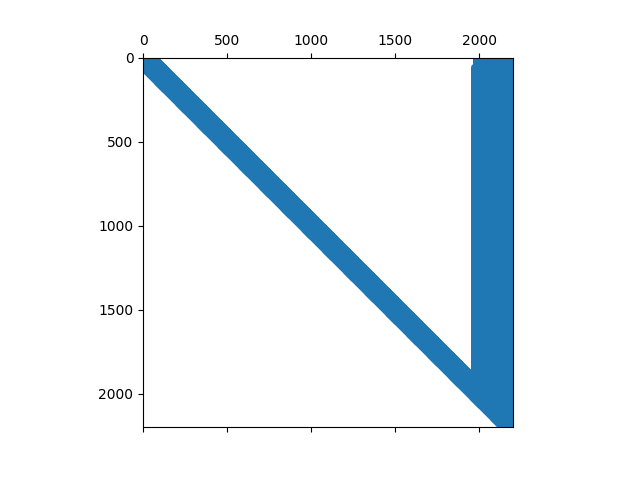
\includegraphics[width=\textwidth]{./results/linear/lu_2d_linear_sparsity.png}
      \caption{\textit{2d\_linear.npz}}
    \end{subfigure}
    \hfill
    \begin{subfigure}[b]{0.45\textwidth}
      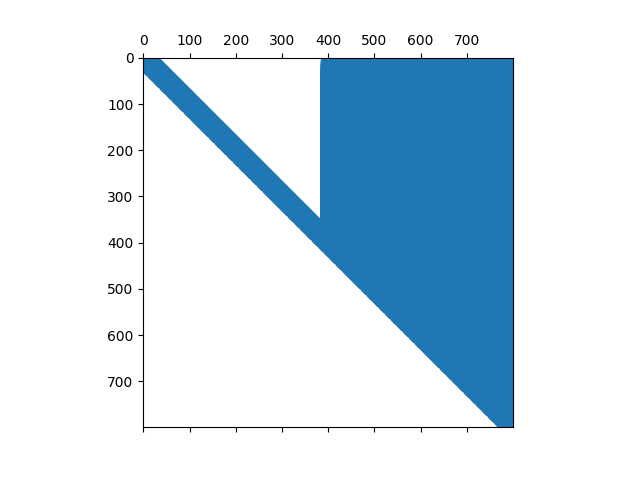
\includegraphics[width=\textwidth]{./results/linear/lu_2d_linear_loop_sparsity.png}
      \caption{\textit{2d\_linear\_loop.npz}}
    \end{subfigure}
    \caption{Sparsity matrices with \textit{lu} method}
  \end{figure}
  
  \item The time for \textit{default} and \textit{qr\_colamd} methods are surprisingly close for both datasets which \textit{could} mean that \textit{spsolve} relies on QR factorization
\end{enumerate}
\subsection{[BONUS] Custom Implementation of Solver}
The custom solver for LU factorization is implemented in the \textit{solve\_lu\_custom\_solver} function in \textit{solvers.py}. The function can be used with the \textit{--method lu\_custom} argument. The execution time on \textit{2d\_linear.npz} is 76 milliseconds which is significantly faster than the \textit{lu.solve} function. The map is shown below:
\begin{figure}[H]
  \centering
  \begin{subfigure}[b]{0.45\textwidth}
    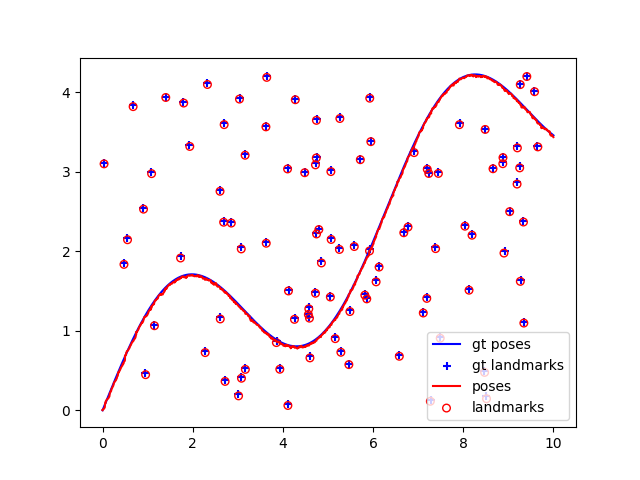
\includegraphics[width=\textwidth]{./results/linear/lu_custom_2d_linear_map.png}
    \caption{Map}
  \end{subfigure}
  \hfill
  \begin{subfigure}[b]{0.45\textwidth}
    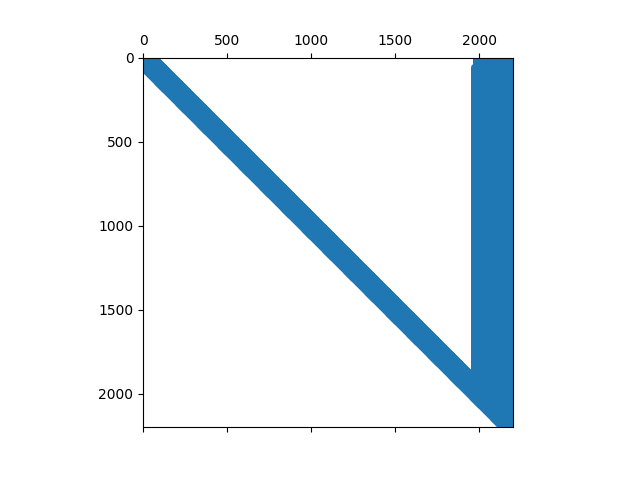
\includegraphics[width=\textwidth]{./results/linear/lu_custom_2d_linear_sparsity.png}
    \caption{Sparsity}
  \end{subfigure}
  \caption{Results with \textit{lu\_custom}}
  \end{figure}
\section{Non-Linear SLAM}
\subsection{Landmark}
\subsubsection{Jacobian}
\[H_l(\mathbf{r}^t, \mathbf{l}^{k}) = \begin{bmatrix}
  \frac{l_y - r_y}{(l_x - r_x)^2 + (l_y - r_y)^2} & \frac{-(l_x - r_x)}{(l_x - r_x)^2 + (l_y - r_y)^2} & \frac{-(l_y - r_y)}{(l_x - r_x)^2 + (l_y - r_y)^2} & \frac{l_x - r_x}{(l_x - r_x)^2 + (l_y - r_y)^2}\\
  \frac{-(l_x - r_x)}{\sqrt{(l_x - r_x)^2 + (l_y - r_y)^2}} & \frac{-(l_y - r_y)}{\sqrt{(l_x - r_x)^2 + (l_y - r_y)^2}} & \frac{l_x - r_x}{\sqrt{(l_x - r_x)^2 + (l_y - r_y)^2}} & \frac{l_y - r_y}{\sqrt{(l_x - r_x)^2 + (l_y - r_y)^2}}\\
\end{bmatrix}\]

\subsection{Results}
\begin{figure}[H]
  \centering
  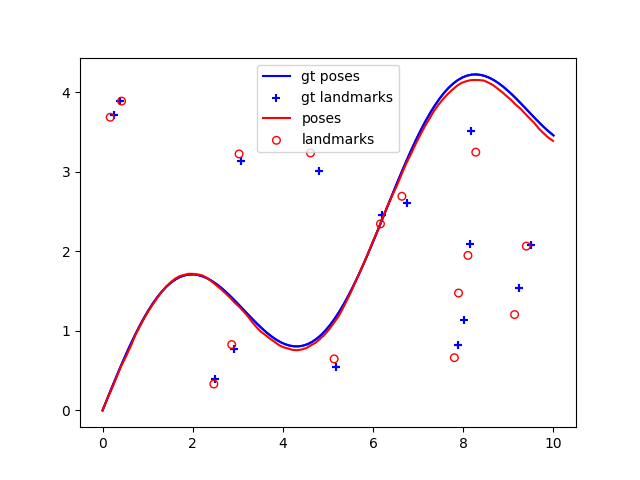
\includegraphics[width=0.8\textwidth]{./results/nonlinear/lu_colamd_2d_nonlinear_map_before.png}
  \caption{Results with \textit{lu\_colamd} optimizer before optimization}
\end{figure}
\begin{figure}[H]
  \centering
  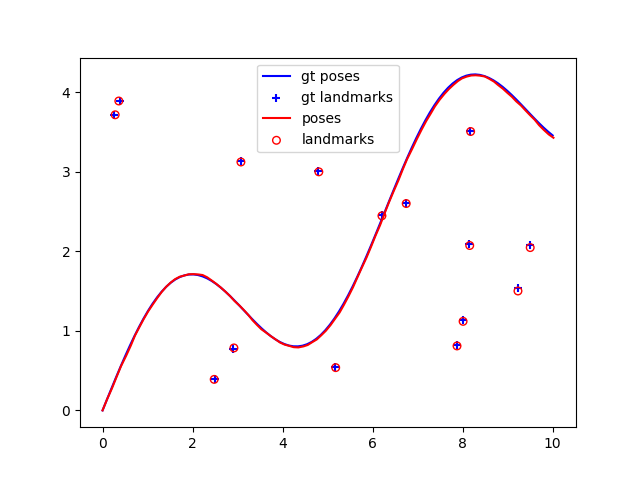
\includegraphics[width=0.8\textwidth]{./results/nonlinear/lu_colamd_2d_nonlinear_map_after.png}
  \caption{Results with \textit{lu\_colamd} optimizer after optimization}
\end{figure}
\subsection{Comparison}
There are two major differences between linear and non-linear optimization approaches
\begin{enumerate}
  \item Linear optimization involves optimization in one single step whereas non-linear optimization requires refinement of solution over several steps resulting in slower execution
  \item In the case of linear optimization problem, the unknown variables that are estimated are the state variables (poses and landmark locations) whereas the unknowns estimated in non-linear optimization problems are the incremental change in the state variables. This requires us to estimate the Jacobian which is time-consuming compared to linear optimization approach.
\end{enumerate}

\end{document}